\section{Results}
\label{resultSection}
\subsection{Compute Resource Utilization}
Section \ref{testReadiness} describes how Istio system resource utilization comparison test is designed with two different environments - single and multiple namespace deployment. In this section test result data and graphs are presented from Grafana with a minimum, maximum and a mean value of CPU and memory consumption over a ten minutes time period for each test. Though the test target is to compare Istio system resource utilization between sidecar and ambient modes, looking at a microservice pod resource utilization in first place gives some initial impression of ambient mode memory efficiency.

\begin{figure}[ht!]
  \centering
  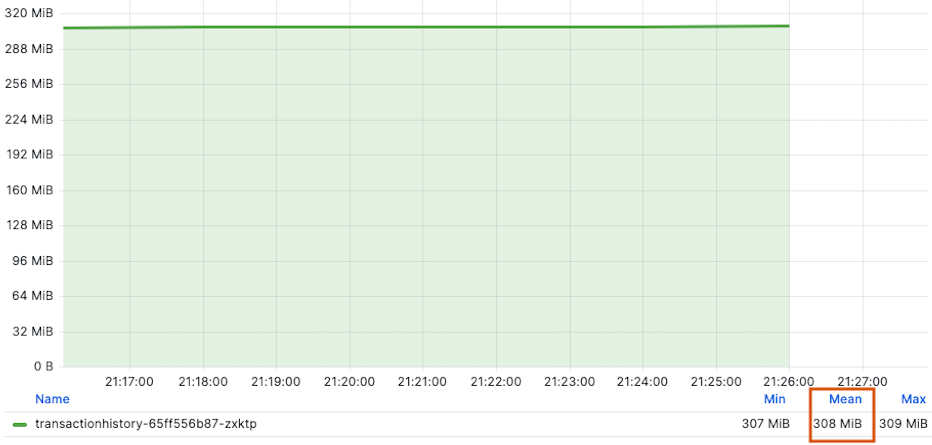
\includegraphics[width=0.73\linewidth]{resources/sidecar-pod-mem.png}
  \caption{Pod Memory Use in Sidecar Mode}
  \label{result:podMemUseSidecar}
\end{figure}

\begin{figure}[ht!]
  \centering
  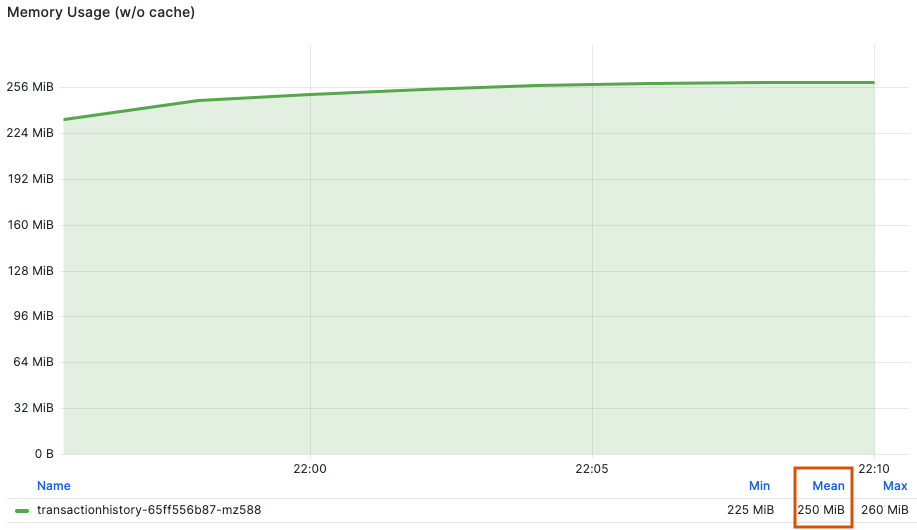
\includegraphics[width=0.73\linewidth]{resources/ambient-pod-mem.png}
  \caption{Pod Memory Use in Ambient L4 Processing Mode}
  \label{result:podMemUseAmbient}
\end{figure}

Figure \ref{result:podMemUseSidecar} and \ref{result:podMemUseAmbient} shows two ten minutes memory usage graph of transaction history microservice pods captured from a single namespace test environment. Looking at the mean or average value of memory usage a significant difference is notice. In sidecar mode the average memory usage is 308 \gls{mib} whereas in ambient mode with L4 processing layer its only 250 \gls{mib}. This result interprets an improvement of 23.2\% memory usage in ambient mode however while comparing the CPU usage there is no noticeable difference found hence the CPU usage details are not shown here. Rest of this section presents the test result graphs from twelve different test cases covering both single and multiple namespace environments. Looking at the graph and test values from bottom right side of the graphics can be intimidating hence before discussing further, Table \ref{allCpuResultsTable} and \ref{allMemResultsTable} summarizes the test results in tabular form. Both the table shows a raw data captured from Grafana with decimal point limited maximum to three places for both CPU and memory utilization.

\begin{table}[ht!]
  \centering
  \begin{tabular}{ |l|c|c|c|c|}
    \hline
    \textbf{Test Environment} & \textbf{\textit{Istio Mode}} & \textbf{\textit{Min}} & \textbf{\textit{Mean}} & \textbf{\textit{Max}} \\
    \textbf{\textit{ }} & \textbf{\textit{ }} & \textbf{\textit{(vCPU)}} & \textbf{\textit{(vCPU)}} & \textbf{\textit{(vCPU)}} \\ \hline
    Single Namespace & Sidecar & 0.020 & 0.107 & 0.125 \\ \hline
    Single Namespace & Ambient L4 & 0.020 & 0.052 & 0.065 \\ \hline
    Single Namespace & Ambient L4+L7 & 0.058 & 0.099 & 0.116 \\ \hline

    Multiple Namespace & Sidecar & 0.230 & 0.403 & 0.463 \\ \hline
    Multiple Namespace & Ambient L4 & 0.075 & 0.208 & 0.235 \\ \hline
    Multiple Namespace & Ambient L4+L7 & 0.124 & 0.245 & 0.344 \\ \hline
  \end{tabular}
  \caption{CPU Usage of Istio System in Different Test Environments}
  \label{allCpuResultsTable}
\end{table}

\begin{table}[ht!]
  \centering
  \begin{tabular}{ |l|c|c|c|c|}
    \hline
    \textbf{Test Environment} & \textbf{\textit{Istio Mode}} & \textbf{\textit{Min}} & \textbf{\textit{Mean}} & \textbf{\textit{Max}} \\
    \textbf{\textit{ }} & \textbf{\textit{ }} & \textbf{\textit{(MiB)}} & \textbf{\textit{(MiB)}} & \textbf{\textit{(MiB)}} \\ \hline
    Single Namespace & Sidecar & 321 & 582 & 610 \\ \hline
    Single Namespace & Ambient L4 & 52.0 & 67.3 & 70.3 \\ \hline
    Single Namespace & Ambient L4 + L7 & 107 & 120 & 124 \\ \hline
    
    Multiple Namespace & Sidecar & 1822.72 & 1843.2 & 1889.68 \\ \hline
    Multiple Namespace & Ambient L4 & 62.4 & 88.6 & 94.5 \\ \hline
    Multiple Namespace & Ambient L4 + L7 & 387 & 461 & 608 \\ \hline
  \end{tabular}
  \caption{Memory Usage of Istio System in Different Test Environments}
  \label{allMemResultsTable}
\end{table}


%%single ns
%sidecar cpu, mem
\begin{figure}[H]
  \centering
  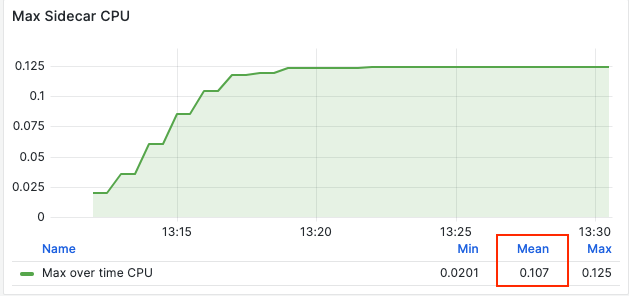
\includegraphics[width=0.8\linewidth]{resources/max-sidecar-cpu.png}
  \caption{CPU Usage of Sidecar Mode in Single Namespace}
\end{figure}

\begin{figure}[H]
  \centering
  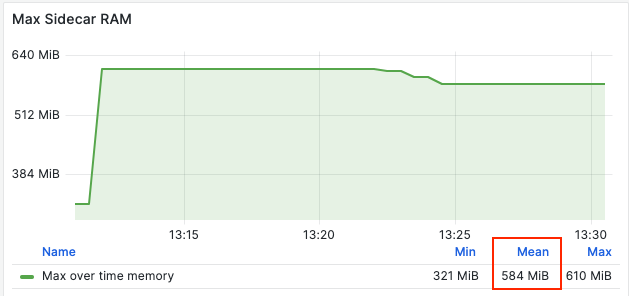
\includegraphics[width=0.8\linewidth]{resources/max-sidecar-mem.png}
  \caption{Memory Usage of Sidecar Mode in Single Namespace}
\end{figure}

%ambient l4 cpu, mem
\begin{figure}[H]
  \centering
  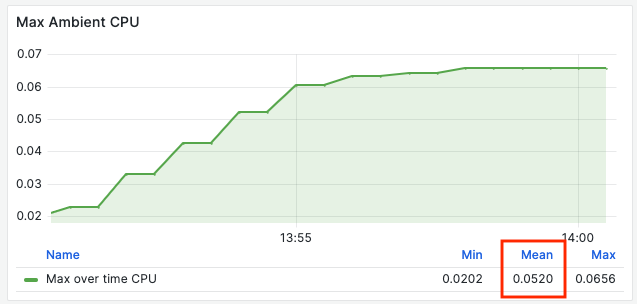
\includegraphics[width=0.8\linewidth]{resources/max-ambient-l4-cpu.png}
  \caption{CPU Usage of Ambient Mode(L4 Only) in Single Namespace}
\end{figure}

\begin{figure}[H]
  \centering
  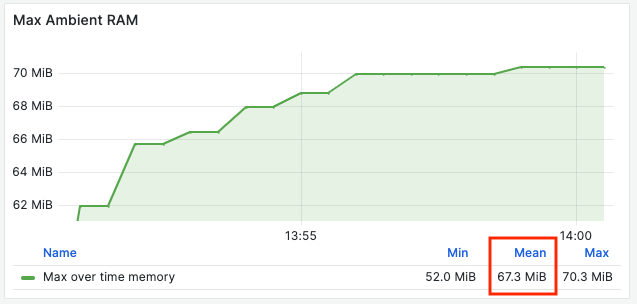
\includegraphics[width=0.8\linewidth]{resources/max-ambient-l4-mem.png}
  \caption{Memory Usage of Ambient Mode(L4 Only) in Single Namespace}
\end{figure}

%ambient l4+l7 cpu, mem
\begin{figure}[H]
  \centering
  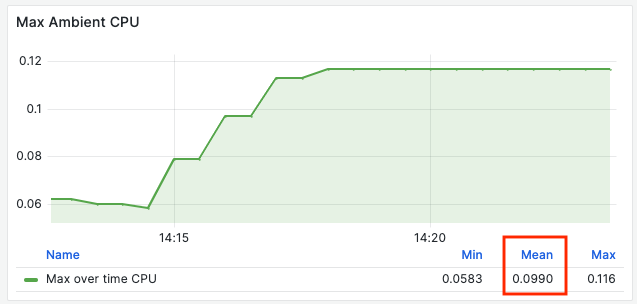
\includegraphics[width=0.78\linewidth]{resources/max-ambient-l4-l7-cpu.png}
  \caption{CPU Usage of Ambient Mode(L4 + L7) in Single Namespace}
\end{figure}

\begin{figure}[H]
  \centering
  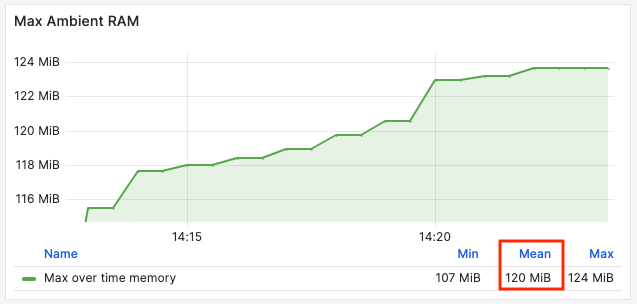
\includegraphics[width=0.8\linewidth]{resources/max-ambient-l4-l7-mem.png}
  \caption{Memory Usage of Ambient Mode(L4 + L7) in Single Namespace}
\end{figure}


%%multi ns
%sidecar cpu, mem
\begin{figure}[H]
  \centering
  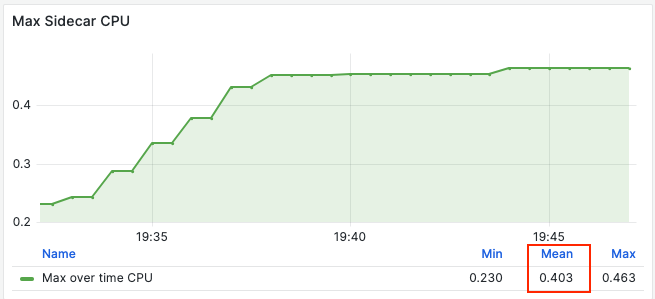
\includegraphics[width=0.8\linewidth]{resources/multi-ns-sidecar-cpu.png}
  \caption{CPU Usage of Sidecar Mode in Multiple Namespace}
\end{figure}

\begin{figure}[H]
  \centering
  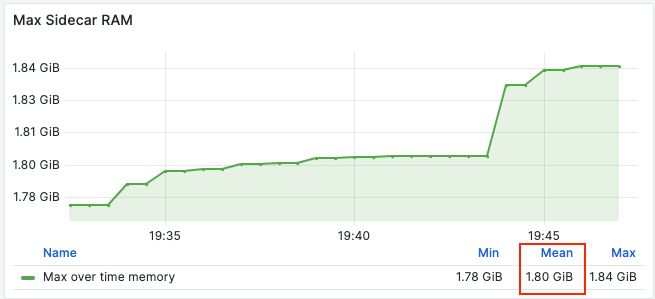
\includegraphics[width=0.8\linewidth]{resources/multi-ns-sidecar-mem.png}
  \caption{Memory Usage of Sidecar Mode in Multiple Namespace}
\end{figure}

%ambient l4 cpu, mem
\begin{figure}[H]
  \centering
  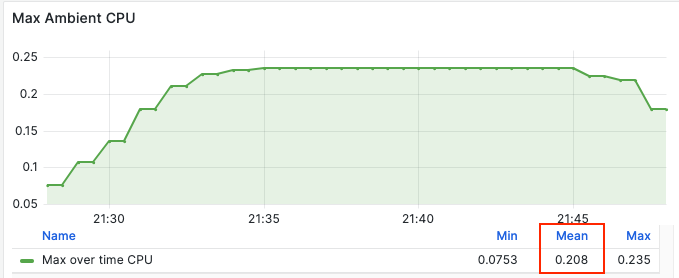
\includegraphics[width=0.8\linewidth]{resources/ambient-multi-ns-l4-cpu.png}
  \caption{CPU Usage of Ambient Mode(L4 Only) in Multiple Namespace}
\end{figure}

\begin{figure}[H]
  \centering
  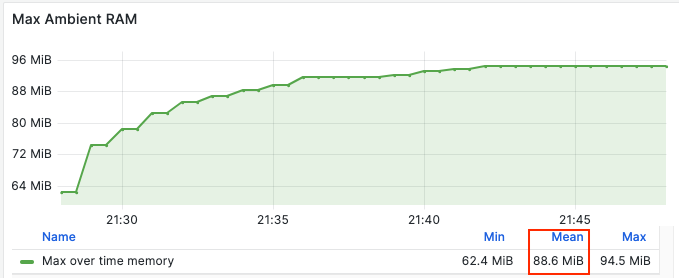
\includegraphics[width=0.85\linewidth]{resources/ambient-multi-ns-l4-mem.png}
  \caption{Memory Usage of Ambient Mode(L4 Only) in Multiple Namespace}
\end{figure}

%ambient l4+l7 cpu, mem
\begin{figure}[H]
  \centering
  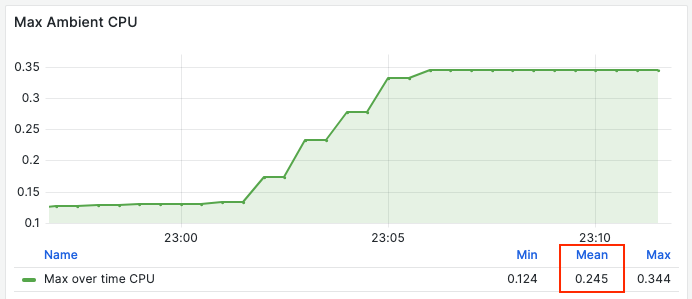
\includegraphics[width=0.85\linewidth]{resources/ambient-multi-ns-l4-l7-cpu.png}
  \caption{CPU Usage of Ambient Mode(L4 + L7) in Multiple Namespace}
\end{figure}

\begin{figure}[H]
  \centering
  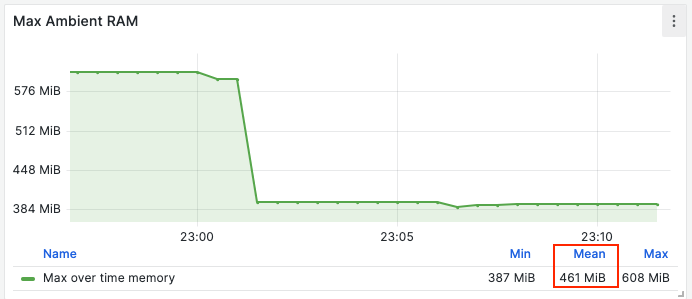
\includegraphics[width=0.85\linewidth]{resources/ambient-multi-ns-l4-l7-mem.png}
  \caption{Memory Usage of Ambient Mode(L4 + L7) in Multiple Namespace}
\end{figure}

With the above test results in place, lets find out the exact performance difference by comparing mean values of CPU and memory usage between sidecar mode, ambient mode with L4 proxy and ambient mode with L4 and L7 proxy. Two different comparison are done between sidecar mode and ambient mode with two different configurations to keep the Ztunnel and Waypoint proxy resource consumption tracked. Table \ref{sidecarCpuVsL4} shows an improvement of 51.4\% in CPU utilization from single namespace test scenario by using 0.107 vCPU by sidecar mode and 0.052 vCPU by ambient mode with L4 processing. In case of multiple namespace test scenario, the difference is 48\% where sidecar mode used 0.403 vCPU and ambient mode with L4 processing used only 0.208 vCPU. Table \ref{sidecarCpuVsL4L7} shows the difference between sidecar and ambient with L4 and L7 processing. The results are 7.4\% improvement in single namespace whereas 39\% improvement in multiple namespace test scenario.

\begin{table}[ht!]
  \centering
  \begin{tabular}{ |l|c|c|c| }
    \hline
    \textbf{Test Environment} & \textbf{\textit{Sidecar}} & \textbf{\textit{Ambient L4}} & \textbf{\textit{Improvement}}\\ \hline
    Single Namespace & 0.107 vCPU & 0.052 vCPU & 51.4\% \\ \hline
    Multiple Namespace & 0.403 vCPU & 0.208 vCPU & 48\% \\ \hline
  \end{tabular}
  \caption{\textit{CPU} Usage Comparison Between Sidecar and Ambient L4}
  \label{sidecarCpuVsL4}
\end{table}


\begin{table}[ht!]
  \centering
  \begin{tabular}{ |l|c|c|c| }
    \hline
    \textbf{Test Environment} & \textbf{\textit{Sidecar}} & \textbf{\textit{Ambient L4 + L7}} & \textbf{\textit{Improvement}}\\ \hline
    Single Namespace & 0.107 vCPU & 0.099 vCPU & 7.4\% \\ \hline
    Multiple Namespace & 0.403 vCPU & 0.245 & 39\% \\ \hline
  \end{tabular}
  \caption{\textit{CPU} Usage Comparison Between Sidecar and Ambient L4 + L7}
  \label{sidecarCpuVsL4L7}
\end{table}

Table \ref{res:sidecarMemVsL4} shows a side by side comparison of memory utilization between Istio sidecar mode and ambient mode with L4 proxy only followed by an improvement percentage. In single namespace environment, sidecar mode uses 584 MiB memory whereas in ambient mode the memory footprint is only 67.3 MiB translating an improvement of 88.47\% in memory usage. Similarly while comparing the results from multiple namespace test environment, the memory utilization is improved in ambient mode by 95.13\% from 1.8 GiB to only 88 MiB. Table \ref{res:sidecarMemVsL4L7} reflects the test comparison result between sidecar mode and ambient mode with both L4 and L7 processing. In single namespace test environment, the improvement is 79.45\% whereas in multiple namespace scenario the efficiency rate is 74.98\%.

\begin{table}[ht!]
  \centering
  \begin{tabular}{ |l|c|c|c| }
    \hline
    \textbf{Test Environment} & \textbf{\textit{Sidecar}} & \textbf{\textit{Ambient L4}} & \textbf{\textit{Improvement}}\\ \hline
    Single Namespace & 584 MiB & 67.3 MiB & 88.47\% \\ \hline
    Multiple Namespace & 1.8 GiB & 88.6 MiB & 95.13\% \\ \hline
  \end{tabular}
  \caption{\textit{Memory} Usage Comparison Between Sidecar and Ambient L4}
  \label{res:sidecarMemVsL4}
\end{table}


\begin{table}[ht!]
  \centering
  \begin{tabular}{ |l|c|c|c| }
    \hline
    \textbf{Test Environment} & \textbf{\textit{Sidecar}} & \textbf{\textit{Ambient L4 + L7}} & \textbf{\textit{Improvement}}\\ \hline
    Single Namespace & 584 MiB & 120 MiB & 79.45\% \\ \hline
    Multiple Namespace & 1.8 GiB & 461 MiB & 74.98\% \\ \hline
  \end{tabular}
  \caption{\textit{Memory} Usage Comparison Between Sidecar and Ambient L4 + L7}
  \label{res:sidecarMemVsL4L7}
\end{table}

\subsection{Operational Complexity}
[TBD]
